\chapter{Progress}\label{progress}
\section{Rheology and Sliding Study}\label{study1}
Building upon the diagnostic ISMIP-HOM experiments in~\cite{Pattyn_2008}, I extend the prognostic experiment F to systematically investigate the combined effects of rheology and basal sliding within this benchmark ice sheet model. The original experiment F included two scenarios: One with a frozen bed (no-slip) and another with linear sliding.
My study expands upon these conditions by also incorporating non-linear rheology. This addition generates four distinct scenarios for comparison:
\begin{compactitem}
    \item{\bf{S1}:} No-slip (frozen) bed + Linear rheology ($n=1$).
    \item{\bf{S2}:} No-slip (frozen) bed + Non-linear rheology ($n=4$).
    \item{\bf{S3}:} Linear sliding + Linear rheology ($n=1$).
    \item{\bf{S4}:} Linear sliding + Non-linear rheology ($n=4$).
\end{compactitem}
To utilise non-linear rheology and still have consistent simulations, I ensure that different model rheologies start from identical initial conditions. The method I follow is based on the re-scaling method by Getraer and Morlighem (2025)~\cite{Getraer_2025}. Their formula ensures that the initial ice viscosity—and therefore strain rates for a given stress—is identical between simulations with different rheologies.
The fundamental model for the deformation of glacial ice and the equations which govern ice flow is Glen's flow law. 
\begin{equation}
\mathbf{\dot{\varepsilon}} \,=\, A_{n}\,\mathbf{\tau}^{n},
\end{equation}
here the $\mathbf{\dot{\varepsilon}}$ is the strain rate, $A_n$ is the rate factor and $\mathbf{\tau}^{n}$ is the stress deviator.
For the non-linear scenarios I am considering $n = 4$, since the assumption of $n = 3$ for ice deformation is not universally supported and values of $n > 3$ have been inferred from real‐world glaciers.
\begin{figure}[H]
    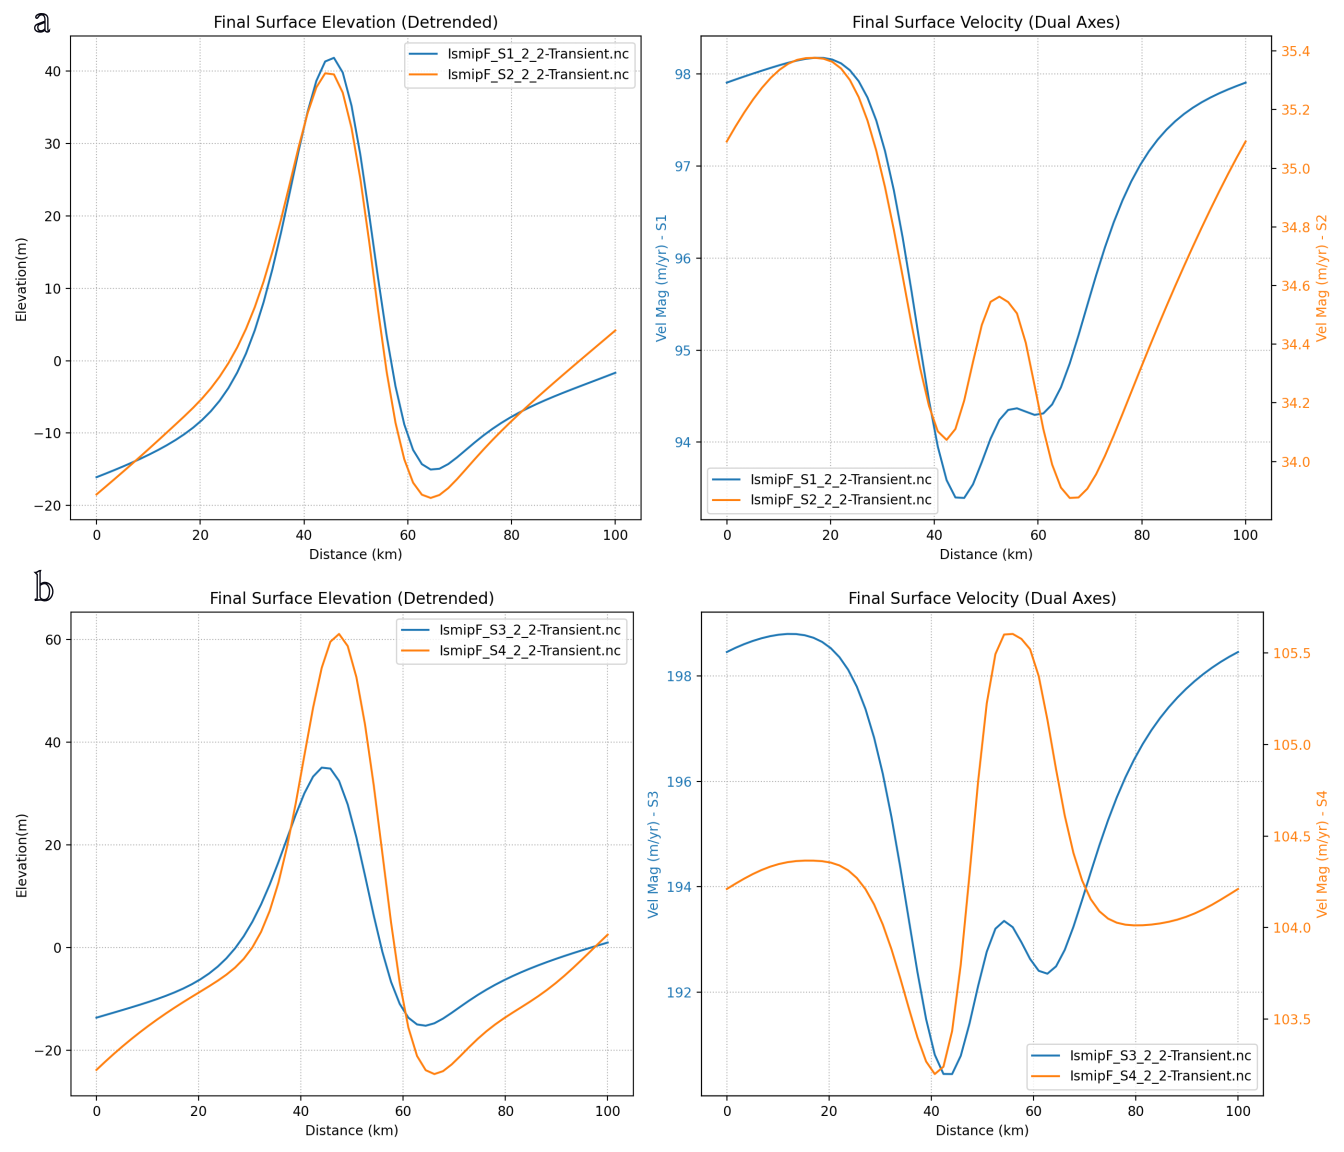
\includegraphics[scale=0.40]{figures/combined_elevation_detrended_surface_velocity_['S1']_['S2']_['S3']_['S4'].png}
    \caption{(a) Final surface elevations and velocities for the original frozen bed Experiment F (S1: linear rheology) and the corresponding transformed to non-linear rheology experiment (S2) (b) Final surface elevations and velocities for the original sliding bed Experiment F (S3: linear rheology) and the corresponding transformed to non-linear rheology experiment (S4).}
    \label{fig:elev_vel_S1_S2_S3_S4}
\end{figure}
The linear results depicted in blue in Figure~\ref{fig:elev_vel_S1_S2_S3_S4} are consistent with the surface elevation and velocities found for Experiment F in~\cite{Pattyn_2008}. Meanwhile, the non-linear scenarios (S2 and S4) shown in orange  represent the first key finding of this analysis. The marked differences in both final surface elevation and velocity compared to the linear counterparts (S1, S3) provide crucial evidence for my first research question (``How does the bed topography manifest on the ice surface?''). Using $n = 4$ leads to a strong non-linear relationship where a small increase in stress yields a much larger increase in deformation. These grid independence results demonstrate that the choice of rheology is an important control on the bed-to-surface signal transfer, implying that a succesful inversion framework like BedSAT must account for non-linear effects.
\newpage
\section{Data Processing, Visualisation and Analysis Tools}\label{analysis_tools}
The core of this study is a time evolution flow simulation of fully grounded ice over 300 years with daily time steps. This simulation is designed to systematically investigate the relationship between basal geometry, ice rheology and flow response by running a series of ISMIP-HOM style experiments~\cite{Pattyn_2008} that can later be analysed in detail with other data processing tools.
\begin{figure}[H]
    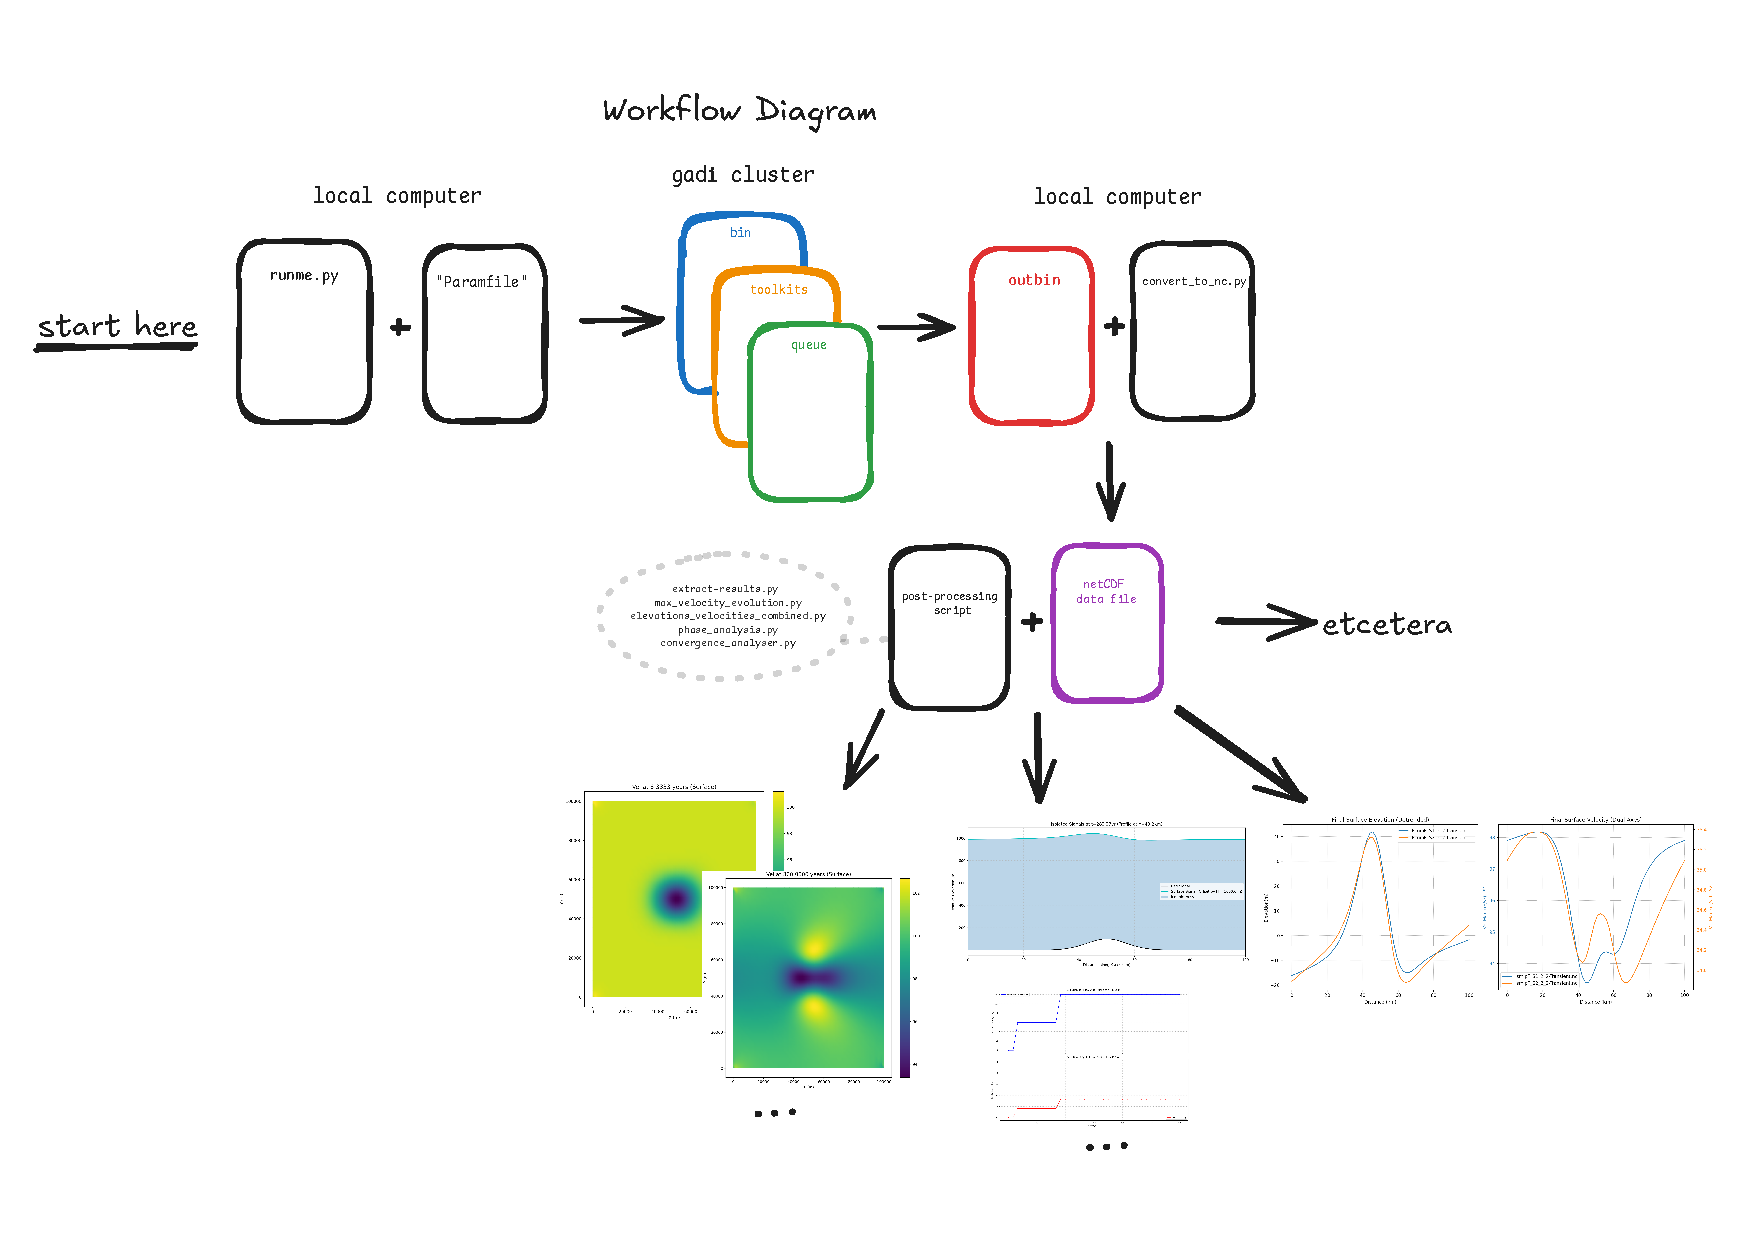
\includegraphics[scale=0.55]{figures/workflow_diagram.pdf}
    \caption{Diagrammatic representation of the current workflow using my ice simulation and analysis suite.}
    \label{fig:workflow}
\end{figure}
The scripts I've developed include a binary file to into NetCDF converter, a transient simulation analyser that generate visualisations of key fields like velocity and pressure. and other additional scripts that create specific scientific analysis and plots.
\subsection{Grid Independence}\label{grid_ind}
Grid optimisation testing involved simulations with 16 distinct mesh resolutions, varying both the horizontal (H) and vertical (V) grid densities independently. The resolution scaling factors tested are $2.0$ (double resolution), $0.5$ (half resolution), $1.0$ (no scaling) and $1.5$ (50\% scaling). I designated the solution from the highest resolution mesh, corresponding to scaling factors of ($H=2.0, V=2.0$) as the reference solution. Refined meshes (either horizontal or vertical) often require smaller time steps to satisfy the Courant-Friedrichs-Lewy (CFL) condition and maintain solver stability. To satisfy this criterion I scaled the time step for each simulation matching the largest resolution factor independently if it was horizontal or vertical scaling.
\begin{figure}[H]
    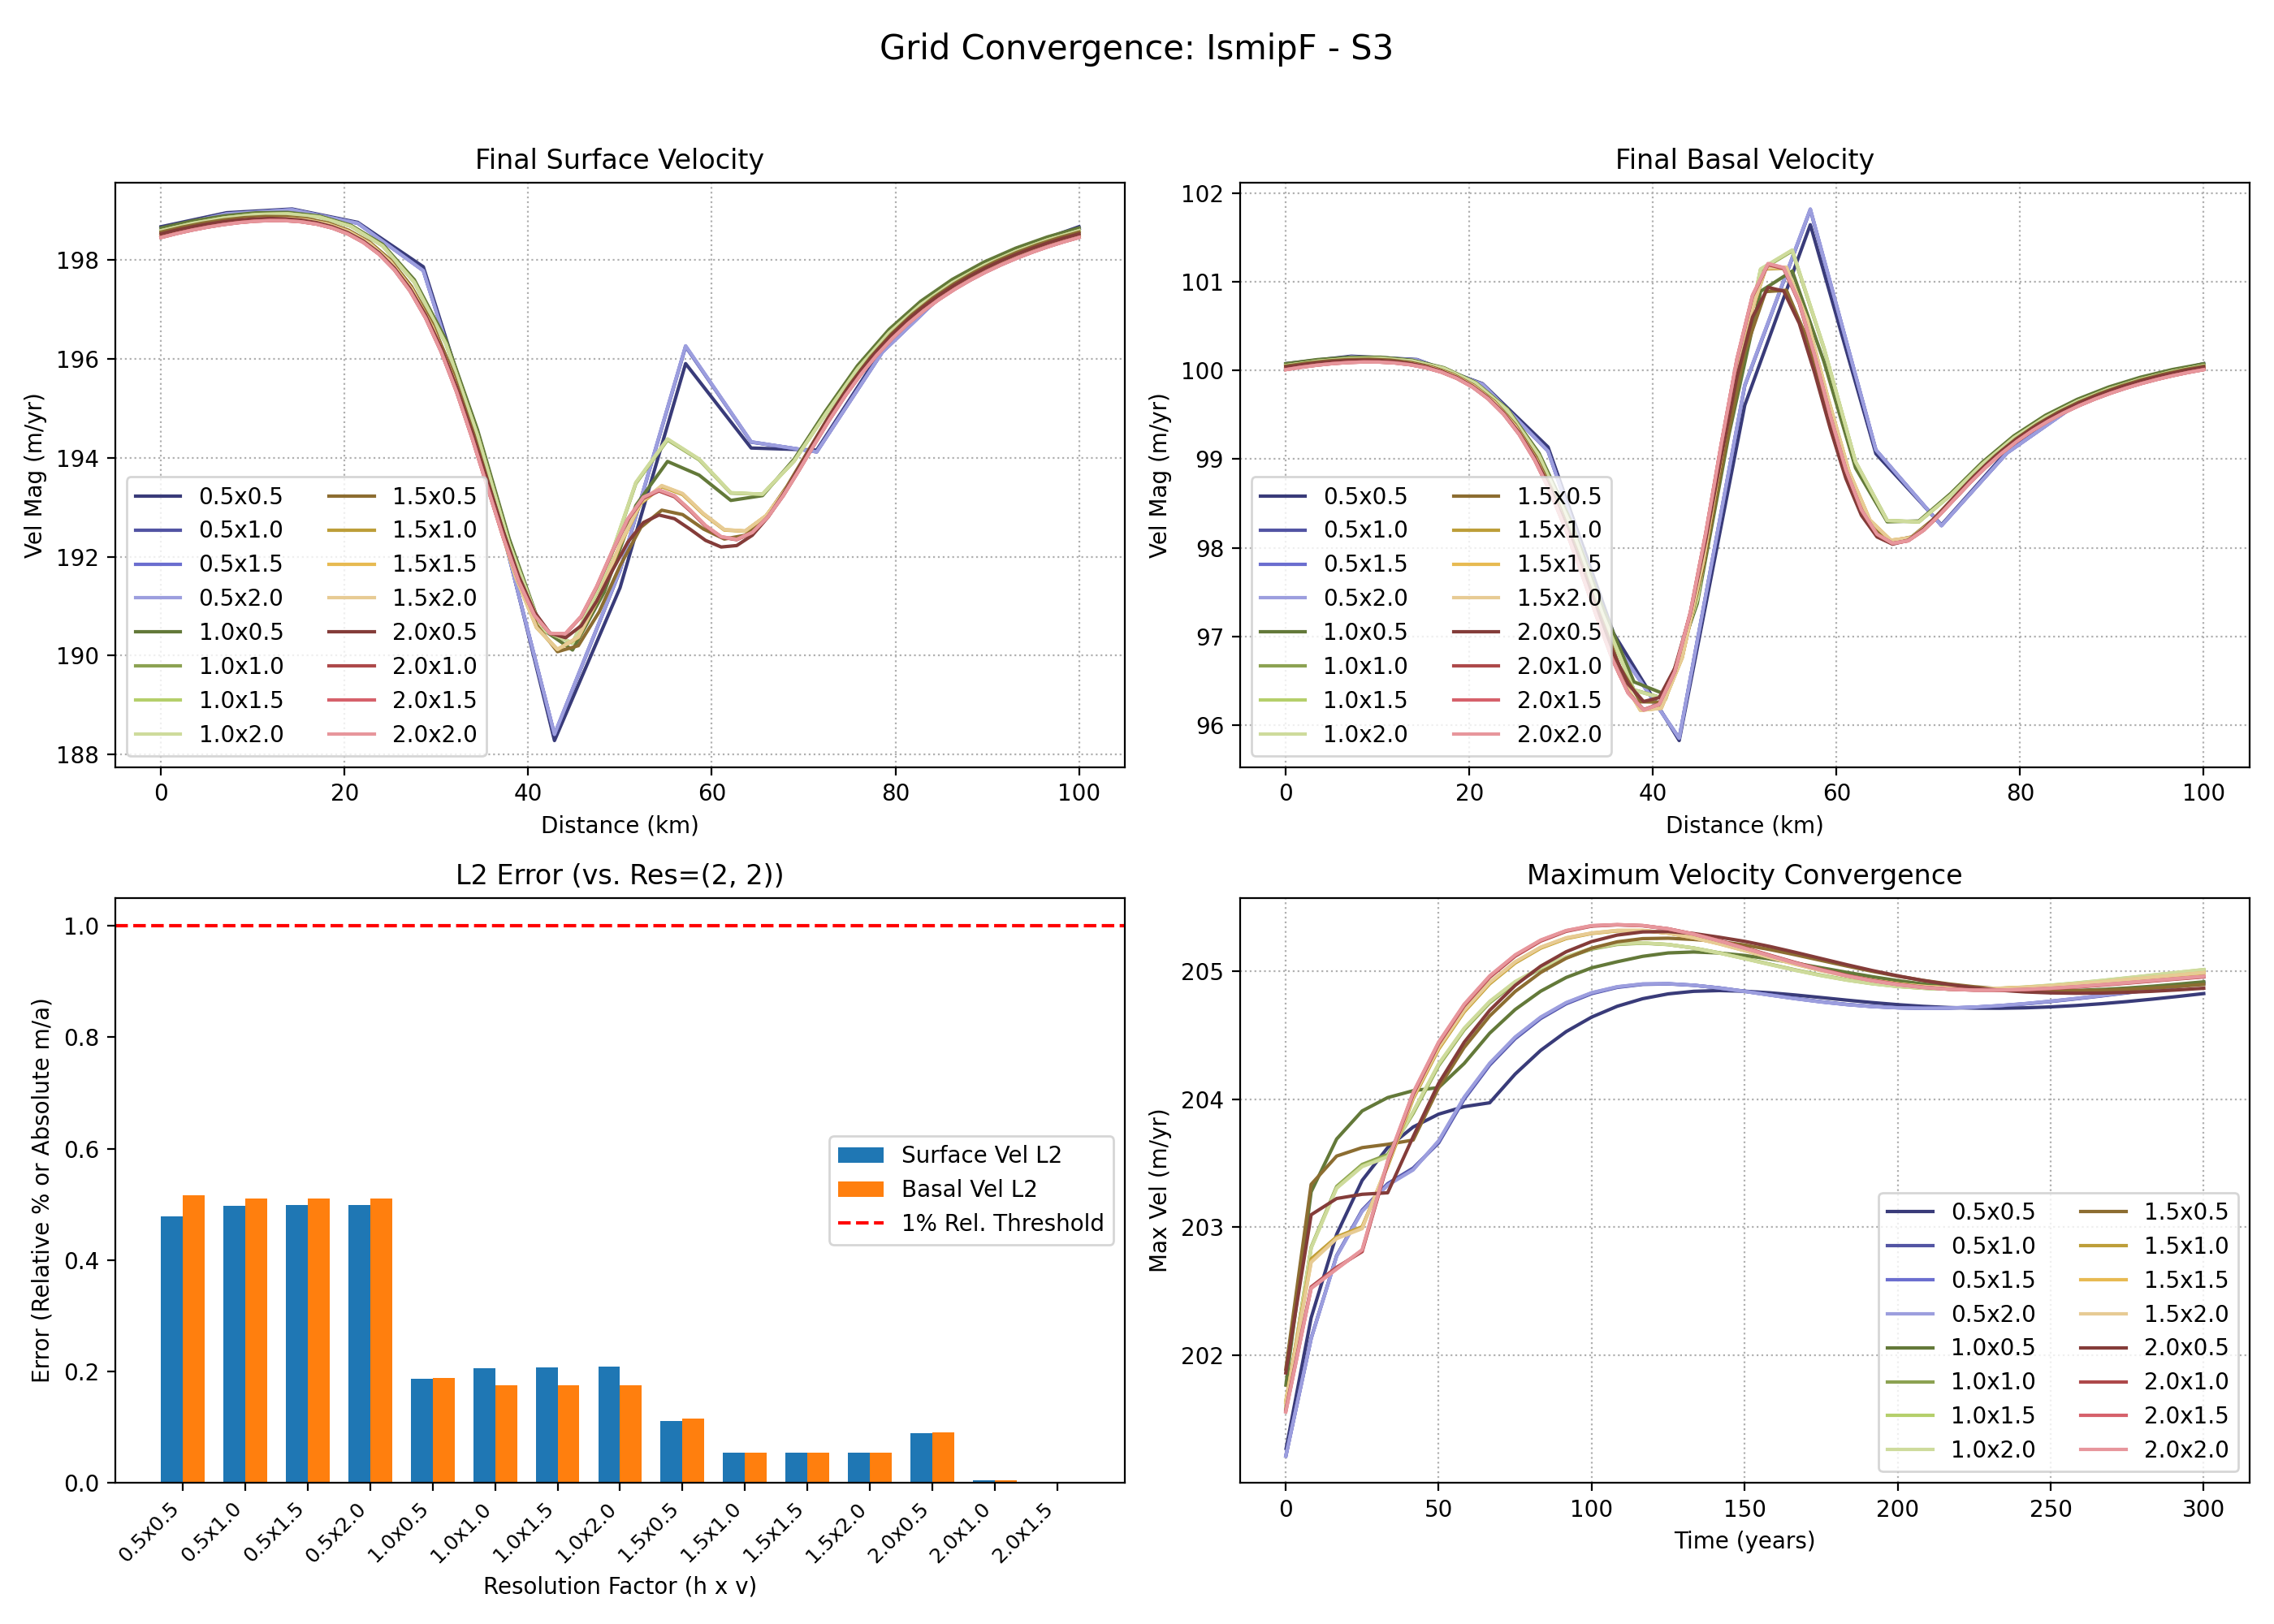
\includegraphics[scale=0.40]{figures/IsmipF_S3_convergence_summary.png}
    \caption{Grid convergence analysis for Scenario S3 (linear sliding, linear rheology, $n=1$). The four panels show: (top-left) final surface velocity profiles and (top-right) final basal velocity profiles for 16 different mesh resolutions; (bottom-left) the L2 relative error of each simulation compared to the highest-resolution mesh ($2.0\times2.0$), with a 1\% relative error threshold indicated by the dashed line; and (bottom-right) the evolution of the maximum velocity over the 300-year simulation period}
    \label{fig:grid_conv_S3}
\end{figure}
\begin{figure}[H]
    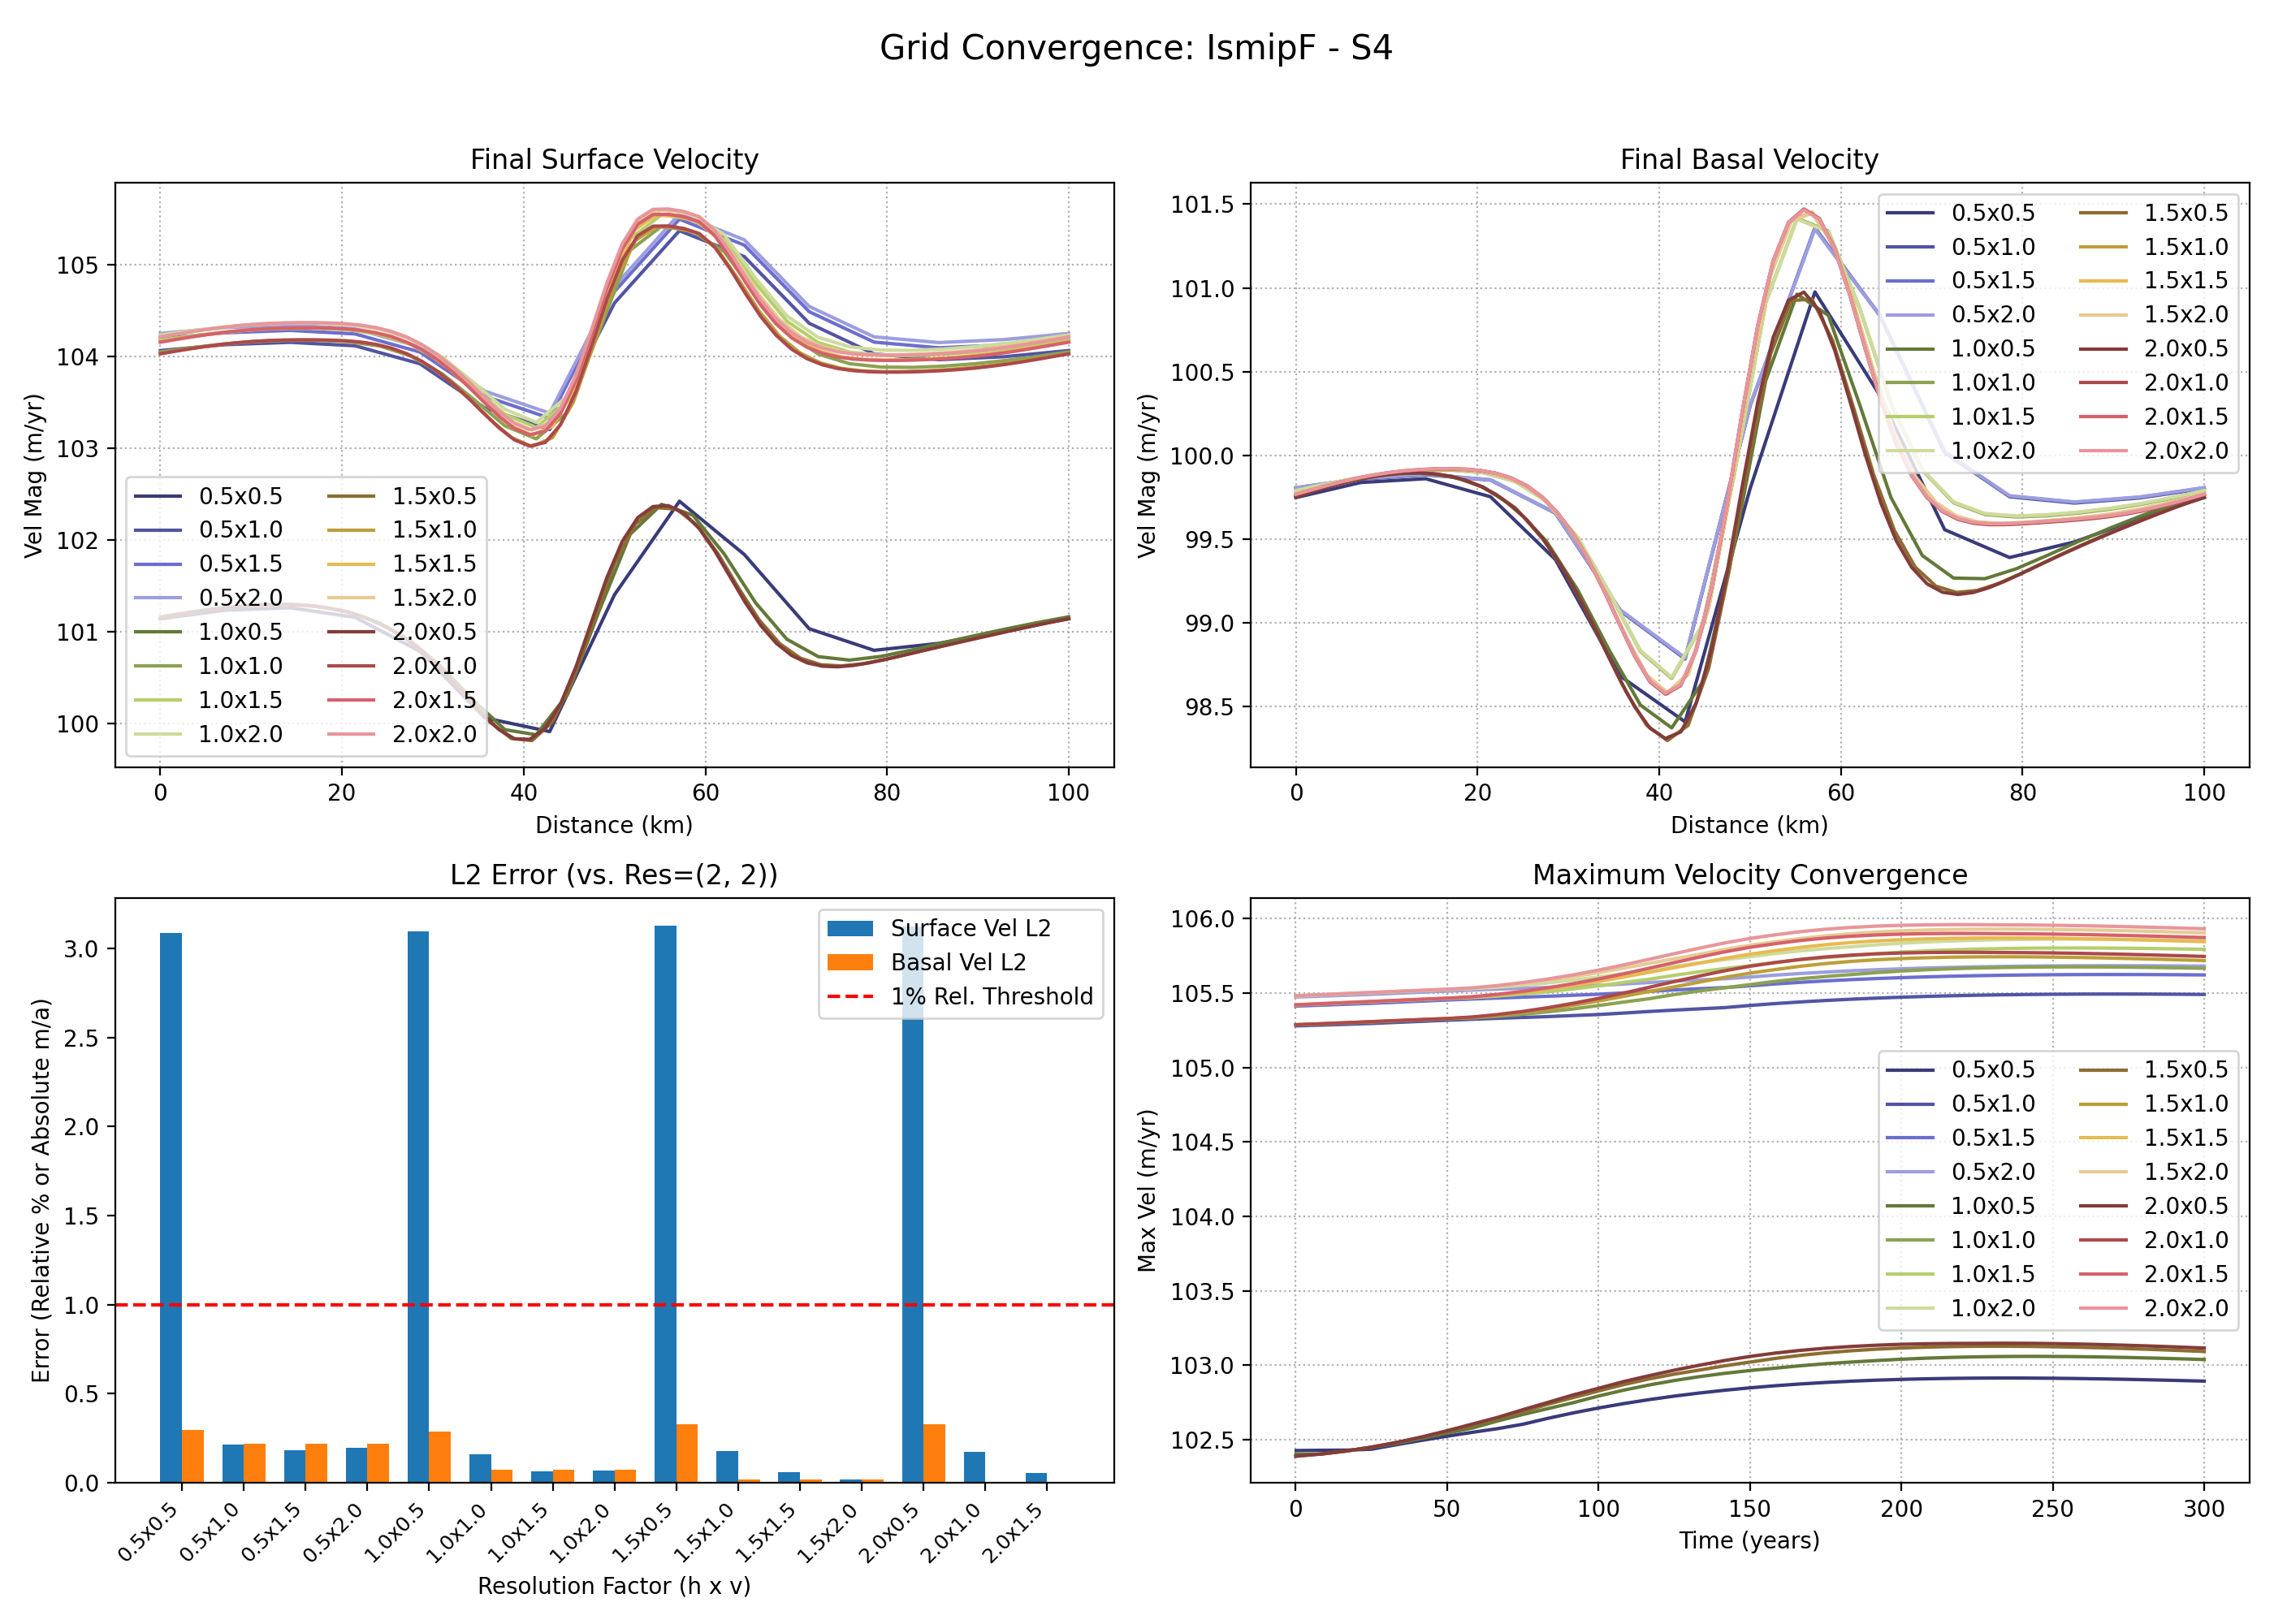
\includegraphics[scale=0.40]{figures/IsmipF_S4_convergence_summary.png}
    \caption{Grid convergence analysis for Scenario S4 (linear sliding, non-linear rheology, $n=4$). Another extension of ISMIP-HOM Experiment F. The convergence analysis demonstrates that non-linear scenarios exhibit high sensitivity to vertical resolution refinement, with low-resolution simulations showing the highest errors (with the relative error threshold only being achieved for simulations using the highest vertical resolution factor (2.0)) and converging to a slower flow state ($\approx~103$ m/a) compared to high-resolution runs ($\approx~106$ m/a).}
    \label{fig:grid_conv_S4}
\end{figure}
The primary metric of this analysis is the L2 relative error, a global, scale-dependent measure that quantifies the overall difference between two solutions. In my analysis, I chose a convergence threshold of $1\%$—since estimates of other uncertainties are expected to be larger than this grid error—when comparing the solutions to the baseline. If the L2 norm of the data is very close to zero (less than $10^{-6}$), the analysis reports the absolute error to avoid division by a tiny, unstable number. Otherwise, it calculates and reports the standard relative error as a percentage.

Convergence analyses show the simulations as most sensitive to vertical resolution. Particularly, non-linear rheology scenarios, where refining vertical resolution produces qualitatively different results. The convergence threshold of 1\% is only achieved for both S2 and S4 in Figure~\ref{fig:grid_conv_S4} with the finest resolution. This high sensitivity underscores the necessity of using converged, high-resolution simulations to generate the training data for BedSAT, ensuring the machine learning model is not learning artefacts from unresolved model physics.

The next phase of my research involves a suite of realistic synthetic bedrock topographies—closely mimicking the conditions found in Antarctica—in order to further inform the development of BedSAT.